\documentclass[fr]{../../../../../../eplexam}

\usepackage{systeme}
\usepackage{cancel}
\usepackage{amsmath,amsfonts,amsthm,bm}
\usepackage{tikz}

\hypertitle{Mécanique des fluides et transferts}{6}{MECA}{1321}{2017}{Juin}{Majeure}
{Martin Braquet}
{Vincent Legat et Grégoire Winckelmans}

\section{Partie Legat}

\begin{figure}[!h]
 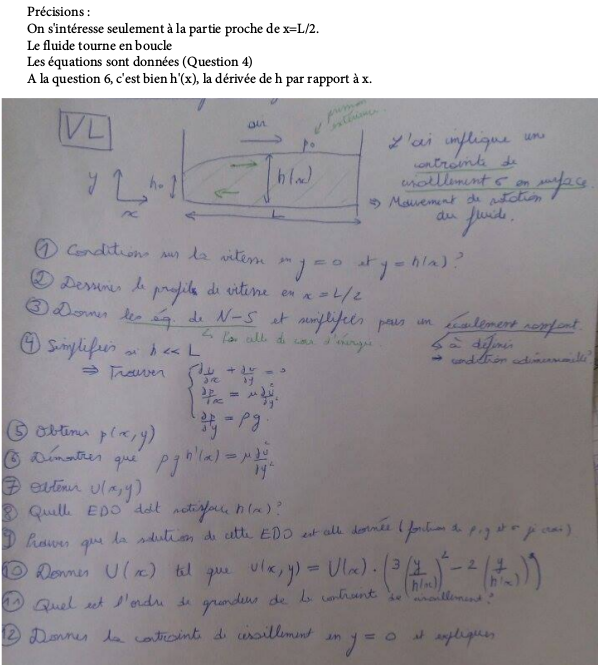
\includegraphics[width=\textwidth]{enonce_VL}
\end{figure}

\begin{solution}

\begin{enumerate}
 \item $u(x,y=0)=0$ et $\bm{\sigma}(x,h(x))\cdot \hat{\bf{e}}_y=(\sigma, \quad -p_0)$
 \item Allure de $u(x=L/2,y)$:
 
 \begin{center}
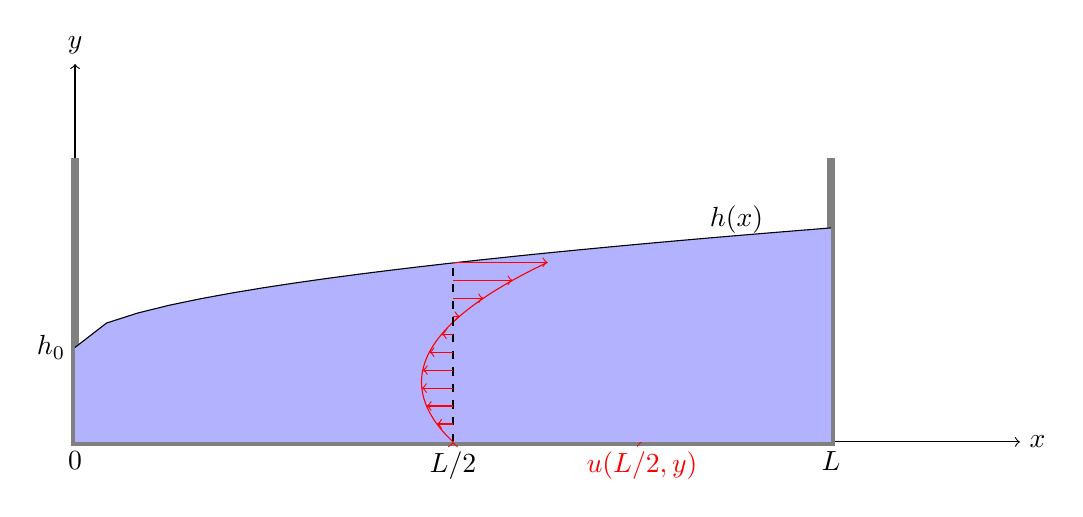
\begin{tikzpicture}[scale=1.2]
 \draw[->] (0,0) -- (0,4) node[above] {$y$};
 \draw[->] (0,0) -- (10,0) node[right] {$x$};
 \draw[line width=1mm, gray] (0,3) -- (0,0) -- (8,0) -- (8,3);
 \draw[->,red] (4,0) -- (6,0) node[below] {$u(L/2,y)$};
 \fill [blue!30, domain=0:8, variable=\y] (0,0) -- plot ({\y},{sqrt(0.2*\y)+1}) -- (8,0) -- cycle;
 \draw[domain=0:1,smooth,variable=\y,red]  plot ({3*\y*\y-2*\y+4},{1.9*\y});
 \draw[domain=0:8, variable=\y] plot ({\y},{sqrt(0.2*\y)+1});
 \draw[dashed] (4,0) -- (4,1.9);
 \draw (7,2.1) node[above] {$h(x)$};
 \draw (0,0) node[below] {0};
 \draw (4,0) node[below] {$L/2$};
 \draw (8,0) node[below] {$L$};
 \draw (0,1) node[left] {$h_0$};
 \foreach \y in {0,0.1,...,1.1} 
       {\draw[->,red] (4,1.9*\y) -- ({3*\y*\y-2*\y+4},1.9*\y);} 
 \end{tikzpicture}
\end{center}
 \item Ecoulement rampant: écoulement pour lequel les termes d'inertie sont négligeables par rapport aux termes visqueux.
 \[
  \systeme*{\frac{\partial u}{\partial x} + \frac{\partial v}{\partial y}=0,
    \cancel{u\frac{\partial u}{\partial x} + v\frac{\partial u}{\partial y}}=-\frac{1}{\rho}\frac{\partial p}{\partial x}+\nu\left(\frac{\partial^2 u}{\partial x^2} + \frac{\partial^2 u}{\partial y^2}\right),
    \cancel{u\frac{\partial v}{\partial x} + v\frac{\partial v}{\partial y}}=-\frac{1}{\rho}\frac{\partial p}{\partial y}+\nu\left(\frac{\partial^2 v}{\partial x^2} + \frac{\partial^2 v}{\partial y^2}\right)-g
    }
 \]

 \item Pour $h<<L$: $$\frac{\partial^2 u}{\partial x^2}=\mathcal{O}\left(\frac{U}{L^2}\right)<<\mathcal{O}\left(\frac{U}{h^2}\right)=\frac{\partial^2 u}{\partial y^2}$$
		    $$\frac{\partial^2 v}{\partial x^2}=\mathcal{O}\left(\frac{V}{L^2}\right)<<\mathcal{O}\left(\frac{V}{h^2}\right)=\frac{\partial^2 v}{\partial y^2}$$
   Donc,
 \[
  \systeme*{\frac{\partial u}{\partial x} + \frac{\partial v}{\partial y}=0,
    -\frac{1}{\rho}\frac{\partial p}{\partial x}+\nu \frac{\partial^2 u}{\partial y^2}=0,
    -\frac{1}{\rho}\frac{\partial p}{\partial y}+\nu \frac{\partial^2 v}{\partial y^2}-g=0
    }
 \]
 La 2e équation montre que $$\mathcal{O}\left(\frac{\Delta p}{\rho L}\right)=\mathcal{O}\left(\nu\frac{U}{h^2}\right)$$
 et donc que $$\frac{1}{\rho}\frac{\partial p}{\partial y}=\mathcal{O}\left(\frac{\Delta p}{\rho h}\right)=\mathcal{O}\left(\nu\frac{UL}{h^3}\right)=\mathcal{O}\left(\nu\frac{VL^2}{h^4}\right)>>\mathcal{O}\left(\nu\frac{V}{h^2}\right)=\frac{\partial^2 v}{\partial y^2}$$
 Ansi,
 \[
  \systeme*{\frac{\partial u}{\partial x} + \frac{\partial v}{\partial y}=0,
    -\frac{1}{\rho}\frac{\partial p}{\partial x}+\nu \frac{\partial^2 u}{\partial y^2}=0,
    -\frac{1}{\rho}\frac{\partial p}{\partial y}-g=0
    }
 \]
 
 \item On résoud la 3e équation,
 \[
  p(x,y)=-\rho g y+f(x)
 \]
  avec $p(x,h(x))=p_0$, donc
  \[
  p(x,y)=\rho g \left[h(x)-y\right]+p_0
 \]
 
 \item On résoud la seconde équation en injectant $p(x,y)$,
  \[
   \mu \frac{\partial^2 u}{\partial y^2}(x,y) = \rho g h'(x)
  \]
 
 \item En intégrant,
 \[
   u(x,y) = \frac{\rho g h'(x)}{2\mu}\left[ y^2+A(x)y+B(x) \right]
 \]
 avec $u(x,y=0)=0$, donc $B(x)=0$.
 
 La condition en surface donne (pour cet écoulement rampant)
 \[
  \bm{\sigma}=2\mu\:\bf{d}-p\:\bf{I}=\mu 
  \begin{pmatrix}
     2\frac{\partial u}{\partial x} & \frac{\partial u}{\partial y}+\cancel{\frac{\partial v}{\partial x}}      \\
    \frac{\partial u}{\partial y}+\cancel{\frac{\partial v}{\partial x}}  & 2\frac{\partial v}{\partial y}        
  \end{pmatrix}
  -p\:\bf{I}=\begin{pmatrix}
     2\mu\frac{\partial u}{\partial x}-p & \mu\frac{\partial u}{\partial y}      \\
    \mu\frac{\partial u}{\partial y}  & 2\mu\frac{\partial v}{\partial y}-p   
  \end{pmatrix}
 \]
 et donc $$\bm{\sigma}(x,h(x))\cdot \hat{\bf{e}}_y=\begin{pmatrix}
     \mu\frac{\partial u}{\partial y}      \\
    2\mu\frac{\partial v}{\partial y}-p   
  \end{pmatrix}=\begin{pmatrix}
     \sigma      \\
    -p_0   
  \end{pmatrix}\quad\Rightarrow\quad \frac{\partial u}{\partial y}(x,h(x))=\frac{\sigma}{\mu}$$
 Ainsi,
 \[
  \frac{\rho g h'(x)}{2\mu}\left[ 2h(x)+A(x) \right]=\frac{\sigma}{\mu} \quad\Rightarrow\quad A(x)=\frac{2\sigma}{\rho g h'(x)}-2h(x)
 \]
 Et finalement
  \[
   u(x,y) = \frac{\rho g h'(x)}{2\mu}\left[ y^2-2h(x)y \right]+\frac{\sigma y}{\mu}
 \]
 
 \item Par conservation du débit à travers l'interface pour tout $x$ proche du centre,
 \begin{equation}
  Q = \int_0^{h(x)}u(x,y) \: dy=0 \quad\Rightarrow\quad \sigma=\frac{2\rho g }{3}h'(x)h(x)
 \end{equation}

 \item Il semblerait que la solution, donnée dans l'énoncé de l'examen, soit
 \[
  h(x) = \sqrt{\frac{3\sigma}{\rho g}x+h_0^2}
 \]
 car elle vérifie bien l'équation (1).

 
 \item En injectant l'équation (1) dans $u(x,y)$,
 
   \[
   u(x,y) = \underbrace{\frac{\rho g h'(x)h^2(x)}{6\mu}}_{U(x)}\left[ 3\left(\frac{y}{h(x)}\right)^2-2\left(\frac{y}{h(x)}\right) \right]
 \]
 
 \item On reprend l'équation (1),
 \[
    \sigma : \mathcal{O}\left(\rho g \frac{h}{L}h \right)=\mathcal{O}\left(\frac{\rho g h^2}{L} \right)
 \]
 \item La contrainte de cisaillement vaut
 \[
    \tau_w=\mu \frac{\partial u}{\partial y}(x,0)=-\frac{\rho g }{3}h'(x)h(x)=-\frac{\sigma}{2}
 \]
 Elle est négative car c'est la force exercée par l'eau sur le sol, donc dirigée vers la gauche. La force exercée par l'eau sur le sol est deux fois plus petite que la force exercée par
 l'air sur l'eau en surface.
 
 \end{enumerate}

\end{solution}

\end{document}
